\documentclass[border=10pt,margin=5pt,tikz,dvisvgm,rgb,utf8]{standalone}
\usepackage{ctex,xeCJK}  % 中文环境
\setCJKmainfont[BoldFont=Source Han Sans SC]{Source Han Serif SC}
\usepackage{calc,fontawesome,forest,smartdiagram,xcolor}
\usetikzlibrary{animations,arrows,automata,graphs,matrix,positioning,shadows,shapes}

\begin{document}
\renewcommand{\baselinestretch}{0.4}

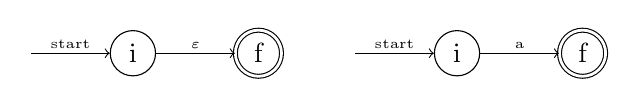
\begin{tikzpicture}
  % \varepsilone
  \node[text width=-3em](EpsilonStart){};
  \node[circle, draw=black, right= of EpsilonStart](EpsilonI){i};
  \node[circle, double, double distance=1pt, draw=black, right= of EpsilonI](EpsilonF){f};
  \path[->]
  (EpsilonStart) edge node[above=-2pt]{\tiny start} (EpsilonI)
  (EpsilonI) edge node[above=-2pt]{\tiny $\varepsilon$} (EpsilonF);

  % subexpr a
  % \node[text width=-3em, below=1.25em of EpsilonStart](SubExprStart){};
  \node[text width=-3em, right=2.5em of EpsilonF](SubExprStart){};
  \node[circle, draw=black, right= of SubExprStart](SubExprI){i};
  \node[circle, double, double distance=1pt, draw=black, right= of SubExprI](SubExprF){f};
  \path[->]
  (SubExprStart) edge node[above=-2pt]{\tiny start} (SubExprI)
  (SubExprI) edge node[above=-2pt]{\tiny a} (SubExprF);
\end{tikzpicture}

\end{document}
